\chapter{Produkt und Reflexion}
\section{Prozess}
\subsubsection{Erstellung der Themenübersichten}
Nachdem der Prototyp der App erstellt war, wurde dieser mit einer Themaübersicht pro Thema erweitert, s. \cref{themen_uebersicht}. In die Themenübersichten kommt man vom Homescreen aus und wählt dort das Unterthema, welches man bearbeiten möchte. 
\begin{figure}
    \centering
    \includegraphics[width=0.28\linewidth]{Picture/themen_uebersicht.jpg}
    \caption{Themenübersicht}
    \label{themen_uebersicht}
\end{figure}
Das Erstellen der Themenübersichten stellte keine besondere Herausforderung dar, diese kam erst mit dem Erstellen der Register der Themenübersichten. Das Register wurde in der Aktivität des Homescreen programmiert und es ist nicht möglich von einer Aktivität auf die Programme einer anderen Aktivität zuzugreifen. Dieses Problem hätte dem Benutzer der App die Navigation in der App erheblich erschwert. \par 
Eine Aktivität hat immer eine eigene Layout-Datei und stellt somit einen eigenen Screen dar. Auf dieser Aktivität können dann mit der Hilfe von Layouts neue Unterseiten entstehen. \par 
Um das Problem zu lösen wurde versucht, eine Technik namens Fragment zu verwenden. Diese Technik erlaubt die Programmierung von Toolbars und Ähnlichem. Zu dieser Technik wurde kein Tutorial gefunden, welches es ermöglicht hätte, diese Technik zu verwenden. Als Lösung wurde in jedes Unterthema das Register neu eingefügt, somit konnte die Navigation erleichtert erreicht werden, ohne das Erlernen einer neuen Programmiertechnik.\par
Nach der Lösung dieses Problemes konnten die Themenübersichten problemlos der App hinzugefügt werden.

\subsubsection{Erstellen der Informationsseiten}

Die Erstellung der Informationsseiten war überwiegend Fleissarbeit, die erledigt werden musste. Hier tauchte ein Problem auf. Das Problem zeigte sich beim Erstellen der aktiven Notrufnummern. Das Problem war, dass man aus der App heraus die Telefon App öffnen können muss und in der Telefon-App bereits die richtige Eingabe erscheinen soll.\par
Um dieses Problem zu bewältigen wurden zwei Techniken verwendet. Die erste Technik ist ein static URI \cite{noauthor_uri_nodate}. Ein static URI ermöglicht der App einen konstanten Zugriff auf die gewünschte Telefonnummer zu haben, welche gebraucht wird, für die zweite Technik. Die zweite Technik ist ein Action Dial Intent \cite{noauthor_intent_nodate}. Ein Action Dial Intent ermöglicht es der App, die Telefon-App zu öffnen. Aufgrund des URI's der dem Intent mitgegeben wird, ist die Telefonnummer bereits eingegeben, wenn die App geöffnet wird.

\subsubsection{Videos}

Die letzten Herausforderungen beim Programmieren der App kamen bei der Implementierung der Videos. Hierbei war der ursprüngliche Plan, Videoviews zu verwenden, da diese speziell für Videos gemacht wurden. Videoviews sind aufwendig zu erstellen und die App braucht dadurch deutlich mehr Speicherplatz. Die Alternative zu einer Videoview war eine Webview. Eine Webview ermöglicht es, den Inhalt einer Website in die App zu integrieren. Diese Funktion wird in der App so verwendet, dass ein Youtube Video in diesem Ausschnitt gezeigt wird. Diese Lösung funktioniert wunderbar, bis auf den Vollbild-Button. Dieser funktioniert nicht, weil die Webview keinen Zugriff auf den gesamten Bildschirm hat und das Video somit nicht im Vollbildmodus abgespielt werden kann. Dieses Problem besteht in der aktuellen Version der App immer noch.

\subsubsection{Testlauf}

Für den Testlauf war geplant, dass drei Personen ohne Pfadierfahrung sich während einer Woche im Selbststudium mit der App das Wissen für die 1. Etappe aneignen. Nach einem Besuch in der Primarschule Conters haben sich 5 Personen bereit erklärt, die App zu testen. Bei der Anfangserhebung am 2.9.2024 war allerdings eine dieser Personen krank und konnte nicht mitmachen. Die andern konnten den Test erfolgreich abschliessen. Am Ende dieser Schulwoche fand die Schlusserhebung statt. Somit gab es vier brauchbare Sets von Anfangs- und Schlusserhebungen.

\subsubsection{Stichprobe}

Die Stichprobe ist die zweite Quelle für ein Feedback. Hier geht es darum von der Zielgruppe ein Feedback zu erhalten. Allen Eltern von Teilnehmern der Pfadi Rhätikon Schiers wurde ein Mail mit der Bitte, die App zu testen gesendet. Dies geschah in der Woche vor den Etappenprüfungen. Nach den Etappen wurde ein weiteres Mail an die Eltern gesendet mit dem Aufruf eine Google Umfrage auszufüllen. Diese Umfrage wurde leider bis jetzt (8.10.2024) nur von vier Personen ausgefüllt.

\subsubsection{Veröffentlichen der App}

Von Anfang an war die Idee, die App nach der Fertigstellung im Google Play Store zu veröffentlichen. Dieses Unterfangen wurde zu Beginn der Arbeit als einfach eingestuft. Diese Einschätzung beruhte allerdings auf veralteten Informationen. Das Veröffentlichen im Google Play Store war eine einfache Aufgabe bis im November 2023, als Google neue Richtlinien für die Veröffentlichung von Apps publizierte. Diese neuen Richtlinien beinhalten neu die Anforderung, einen geschlossenen Testlauf mit 20 Testern zu machen, um eine App veröffentlichen zu können. Nach einigen Umfragen im eigenen Umfeld wurden einige Tester gefunden. Es waren aber nicht genug Leute, daher wurde die Suche nach Testern ins Internet verschoben. \par
Der erste Versuch war, über Reddit an Tester zu kommen. Hier gibt es ganze Subreddits nur für die Suche von 20 Testern für diesen Testlauf vom Google Play Store. Es funktioniert nach dem Prinzip: Ich teste deine App und du meine. Bei diesem Ansatz gab es allerdings ein Problem mit dem Link zur App und es musste auf eine neue Strategie gesetzt werden. Die neue Strategie basiert auf der App Testers Community. Testers Community erlaubt es einem genau wie auf Reddit andere Apps zu testen und die eigene testen zu lassen mit dem Unterschied, dass es hier keine Probleme mit falschen Links gibt. Wenn diese Lösung nun funktioniert, wird die App bis zur Abgabe des korrigierten Berichtes im Google Play Store erhältlich sein.

\newpage

\section{Endprodukt}

Das Produkt dieser Maturaarbeit ist eine Android App namens Pfaditechnik. Die App beinhaltet Informationen über die Pfaditechniken Pionier, Samariter, Übermittlung, Karte und Kompass, Natur, Pfadigeschichte und das Packen eines Rucksacks. Es sind die Informationen, welche man braucht um eine 1. Etappenprüfung bei der Pfadi Rhätikon Schiers zu bestehen. Um zu den Informationen zu gelangen, erreicht man zuerst eine Themenübersicht. Die Themenübersicht erscheint durch das Klicken der Themen Symbole auf dem Homescreen (\cref{fig:homescreen}). Alternativ kann man das Register verwenden (\cref{fig:register}). Um zum Register zu kommen, muss man auf den Hamburgerbutton in der oberen linken Ecke klicken. Vom Register aus, kann man zu allen Themen gelangen, speziell zum Thema Sonstiges, welches nur über das Register erreichbar ist. Das Register kann von jedem Ort in der App geöffnet werden. Von der Themenübersicht kann man auf die einzelnen Informationsseiten zugreifen (\cref{fig:themen_uebersicht}). Ausserdem gibt es bei den Themenübersichten und bei den Informationsseiten nun einen Homebutton, welcher zurück zum Homescreen führt. Auf den Informationsseiten sind die Informationen zu den einzelnen Unterthemen (\cref{fig:informationsseite}). Die Informationen sind entweder in Text, Bild oder Videoform dargestellt. 
\begin{figure}[!hp]
    \centering
    \begin{minipage}[b]{0.4\textwidth}
        \centering
        \includegraphics[width=0.7\textwidth]{Picture/homescreen.jpg}
        \caption{Homescreen}
        \label{fig:homescreen}
    \end{minipage}
    \begin{minipage}[b]{0.4\textwidth}
        \centering
        \includegraphics[width=0.7\textwidth]{Picture/register.jpg}
        \caption{Register}
        \label{fig:register}
    \end{minipage}

    \vspace{0.05\textwidth}
    
    \begin{minipage}[b]{0.4\textwidth}
        \centering
        \includegraphics[width=0.7\textwidth]{Picture/themen_uebersicht.jpg}
        \caption{Themenübersicht}
        \label{fig:themen_uebersicht}
    \end{minipage}
    \begin{minipage}[b]{0.4\textwidth}
        \centering
        \includegraphics[width=0.7\textwidth]{Picture/inhaltsseite.jpg}
        \caption{Informationsseite}
        \label{fig:informationsseite}
    \end{minipage}
\end{figure}
Die Videos werden indirekt über YouTube dargestellt, was bedeutet, dass man eine aktive Internetverbindung benötigt, um auf die Videos zugreifen zu können. Um von den Informationsseiten wieder zur Themenübersicht zu gelangen, kann man auf den Titel des Themas drücken oder über das Register gehen.
\newpage

\section{Reflexion und Ausblick}

\subsection{Reflexion zum Produkt}

Das Endprodukt und der Entwurf stimmen gut miteinander überein. So hat sich zum Beispiel das Design der App nur wenig verändert. Das Design finde ich passend, da es überwiegend aus der Farbe Grün besteht, welche oft mit Natur assoziiert wird, welche wiederum eine wichtige Rolle in der Pfadi spielt. Die Navigation in der App entspricht genau der Navigation, welche im Entwurf geplant war. Die Navigation ist meiner Meinung nach intuitiv und einfach gehalten, so kann man von jedem Ort in der App mit maximal 3 Klicks an jeden anderen Ort gelangen. Die Informationen in der App sind so dargestellt, wie von Anfang an geplant. Die Darstellung in Form von Text, Bild und Video hat die Nutzung der App vielseitiger gemacht. Die Implementierung der Videos ist jedoch eine andere, als zu Beginn geplant. Die aktuelle Implementierung hat zwar viele Vorteile, nimmt der App aber die Fähigkeit, alles offline zur Verfügung zu stellen. \par
Das Produkt hat noch einige Probleme. Auf einigen Geräten wird zum Beispiel die Schrift nicht in Schwarz sondern einem Grauton dargestellt, dies macht die Texte praktisch unleserlich. Der Grund dafür ist mir unerklärlich, da ich die Textfarbe explizit auf Schwarz gestellt habe. Die App kann auch noch nicht im Querformat verwendet werden, dies ist allerdings absichtlich so gemacht, da die App für das Hochformat programmiert wurde und in den meisten Fällen Hochformat mehr Sinn macht. Im Bereich der Programmierung hat die App noch Verbesserungspotential, zum Beispiel der Code des Registers nochmals überarbeitet werden. Das Register funktioniert zwar, aber wenn die App erweitert werden soll, ist ein grosser Aufwand nötig, um das Register auf diese neuen Bereiche zu expandieren. 

\subsection{Reflexion zum Projekt}

\subsubsection{Projektauftrag}

Der Projektauftrag wurde aus meiner Sicht klar erfüllt. Ich habe eine Android App entwickelt, welche es Eltern und Pfadis ermöglicht sich selbst die Pfaditechniken der ersten Etappe beizubringen, das Einzige was nicht erreicht wurde, ist das Veröffentlichen der App. Die Veröffentlichung der App sollte bis zur nächsten Abgabe vollzogen sein. An der Ausgangssituation hat sich im Verlauf des Projekts sehr wenig verändert und die Nutzer der App gibt es. Die App wurde zur Vorbereitung auf die Etappenprüfungen 2024 zur Verfügung gestellt und war ein mässiger Erfolg. Die App wurde meines Wissens nach mindestens von den vier Personen, welche die Umfrage der Stichprobe ausgefüllt haben, benutzt. Die Information über die Existenz meiner App kam Pfadileitern anderer Abteilungen zu Ohren, welche mich anfragten, ob sie die App ebenfalls haben könnten, um sie für ihre eigene Pfadi zu brauchen. Daraus ziehe ich den Schluss, die App ist ein Erfolg und hat ihre Nische gefunden.

\subsubsection{Projektziele}

Das erste Projektziel zur Erstellung einer App, welche alle Bereiche der ersten Etappe abdeckt, wurde erreicht. Die erstellte App beinhaltet alle Informationen, welche benötigt werden, um die erste Etappe zu bestehen. Zusätzliche Funktionen wie ein interaktiver Zeitstrahl oder ähnliches, gibt es noch nicht in der App, aber diese Funktionen sind nicht wesentlich, um die erste Etappe zu bestehen. \par
Der Testlauf wurde wie geplant vor den Stichproben durchgeführt. Als Testpersonen fungierten vier freiwilige Personen der Primarschule Conters. Die Anfangserhebung fand am 2.9.2024 statt und die Testpersonen erhielten an diesem Tag Zugriff zu der App. Bis zur Schlusserhebung bekamen diese Personen den Auftrag sich eine Woche lang täglich 15 min mit der App auseinanderzusetzen. Am 6.9.2024 fand die Schlusserhebung mit einem Feedbackteil statt. Die Ergebnisse der Tests fielen durchwegs positiv aus. Sie wurden in \cref{fig:fortschritt} dargestellt. Die maximale Punktzahl war 37 Punkte. Aufgrund der kleinen Datenmenge, kann kein genauer Schluss gezogen werden, aber da sich jede Testperson im Durchschnitt um 12.25 Punkte verbessert hat, schliesse ich aus dem Testlauf, dass die App ihre Funktion erfüllt.

\begin{figure}[ht]
    \centering
    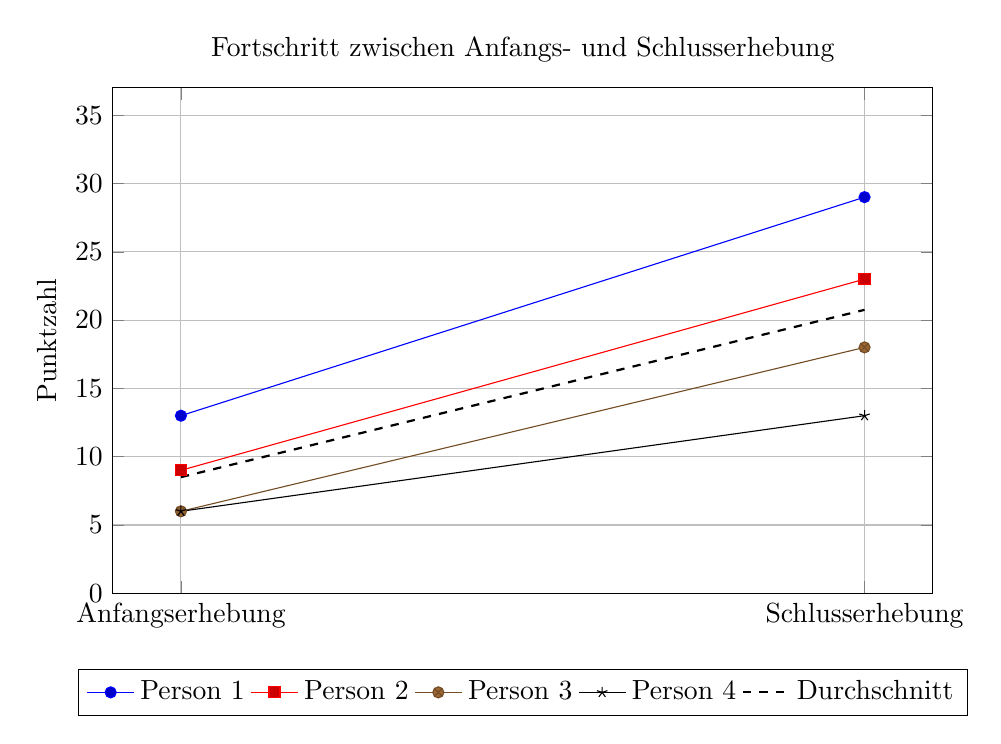
\begin{tikzpicture}
        \begin{axis}[
            title={Fortschritt zwischen Anfangs- und Schlusserhebung},
            ylabel={Punktzahl},
            xtick={1, 2},
            xticklabels={Anfangserhebung, Schlusserhebung},
            ymin=0, ymax=37,
            legend style={at={(0.5,-0.15)}, anchor=north, legend columns=-1},
            grid=major,
            width=12cm,
            height=8cm
        ]

        \addplot coordinates {(1,13) (2,29)};
        \addlegendentry{Person 1}

        \addplot coordinates {(1,9) (2,23)};
        \addlegendentry{Person 2}

        \addplot coordinates {(1,6) (2,18)};
        \addlegendentry{Person 3}

        \addplot coordinates {(1,6) (2,13)};
        \addlegendentry{Person 4}

        \addplot[color=black, thick, dashed] coordinates {(1,8.5) (2,20.75)};
        \addlegendentry{Durchschnitt}

        \end{axis}
    \end{tikzpicture}
    \caption{Punkteverlauf der vier Personen und Durchschnitt}
    \label{fig:fortschritt}
\end{figure}

Das Feedback aus der Schlusserhebung war überwiegend positiv und alle Testpersonen haben sich in der App gut bis sehr gut zurecht gefunden. Auch die Informationen in der App fanden alle gut dargestellt. Zwei Verbesserungswünsche kamen zum Vorschein. Die erste Verbesserung wären Bilder in die man hereinzoomen kann und das Andere wären Spiele, um so spielend das Wissen erlernen und festigen zu können. \par
Das letzte Projektziel mit den Stichproben war das Projektziel, welches am schlechtesten erreicht wurde. Die Stichprobe wurde nach Absprache mit dem Coach umgeplant. So wurden nun nicht mehr 5 Pfadis und 5 Eltern spezifisch gefragt, die App zu testen, sondern es wurde eine Mail an alle Eltern geschrieben mit der Bitte die App zu testen. Die Mail wurde eine Woche vor den Etappenprüfungen versendet. Eine Woche später wurde dann eine zweite Mail versendet mit der Bitte, dass alle Personen, welche meine App getestet haben mir bitte Feedback geben sollen. Die Umfrage, welche in dem Mail enthalten war, wurde nur von 4 Personen ausgefüllt. Die Rückmeldungen von diesen Personen waren überwiegend positiv \cite{noauthor_feedback_nodate}. Ein Verbesserungsvorschlag war, kleine Tests einzufügen, damit die Eltern ihre Kinder testen können, um sie optimal auf die Etappen vorzubereiten.

\subsubsection{Lernziele}

Das erste Lernziel zur Erlernung der Programmiersprache Java wurde übertroffen. Ich kann im Nachhinein sagen, dass für die Programmierung einer App kein tiefes Verständnis von Java nötig ist. Für die App wurden praktisch nur Verzweigungen, Variablen und Klassen und Objekte verwendet. Schlaufen und die wichtigsten Datentypen waren für das Programmieren irrelevant. Das Verständnis von Klassen und Objekten war zwar von Vorteil bei der Programmierung, aber keinesfalls notwendig. Etwa die Hälfte des Codes für die App wurde in der Programmiersprache XML geschrieben. XML wird verwendet, um Objekte auf dem Bildschirm zu erstellen und ihnen ihre Eigenschaften zu geben, Java gibt diesen Objekten dann ihre Funktionen. Da XML eine einfache Programmiersprache ist, hat mir dies keine Probleme bereitet. \par
Das zweite Lernziel zu den Kenntnissen in Android Studio und der Veröffentlichung im Google Play Store, wurde teilweise erreicht. Das Erlernen der erforderlichen Kenntnisse in Android Studio stellten keine grosse Herausforderung dar. Die erwarteten Kenntnisse entsprachen genau dem Niveau, das benötigt wurde, um diese App zu programmieren. Das Einzige, was das Programmieren in Android Studio noch vereinfacht hätte, wären Informationen über Fragmente gewesen, aber es hat auch ohne funktioniert. Die Veröffentlichung hat nicht funktioniert, so ist die App zum aktuellen Zeitpunkt noch nicht im Google Play Store veröffentlicht aufgrund von Richtlinienänderungen von Google, welche das Aufladen von Apps deutlich erschweren. \par
Das dritte Lernziel zur Verbesserung der \LaTeX -Kentnisse, um die Maturaarbeit in \LaTeX zu schreiben, wurde erreicht und hat mir die Formatierung der Arbeit deutlich vereinfacht. Meine \LaTeX -Kenntnisse reichen aus, um die Maturaarbeit in Overleaf mit \LaTeX zu schreiben und so durch das Programm Zeit zu sparen und meiner Meinung nach einen optisch schöneren Bericht zu schreiben.

\subsubsection{Verbesserungen}

Das Projekt war in meinen Augen ein Erfolg. Jedoch gibt es noch einiges was verbessert werden könnte. Der Zeitplan wurde in Form von Userstories gemacht, was mir die Möglichkeit gab einen flexiblen Zeitplan zu haben. Das war für mich sehr nützlich, hatte aber zur Folge, dass die meiste Arbeit in der Vorwoche der Abgabe stattgefunden hat, da mir fixe Zwischentermine fehlten. \par
Die Feedbackgewinnung ist ein weiterer Teil des Projekts, der sich verbessern lässt. Der Testlauf hat gut funktioniert, aber da es nur 4 Personen waren, habe ich zu wenig Daten, um genaue Schlüsse zu ziehen. Die Stichprobe hat mässig funktioniert, hier war ebenfalls die fehlende Datenmenge das Problem. Nur 4 Personen haben die Feedbackumfrage ausgefüllt. Ich denke es wäre passender gewesen, wie geplant, 5 Eltern und 5 Pfadis spezifisch zu fragen, ob sie meine App testen könnten. Somit hätte ich sicher 10 Feedbacks gehabt und wäre nicht auf den Goodwill aller Eltern angewiesen gewesen.

\subsection{Ausblick}

Die App wird wahrscheinlich in Zukunft weiterhin genutzt werden. Sei es nun von Eltern, welche ihre Kinder auf die Etappen vorbereiten, von Pfadis, welche sich selbst die Pfaditechniken beibringen oder von Leitern, die schnell etwas in der App nachschauen wollen. Die App wird weiterhin von mir mit Updates versehen. Es ist geplant den Stoff der 2. und 3. Etappen auch noch in die App zu integrieren. Das Feedback und die Verbesserungsvorschläge des Testlaufs und der Stichproben möchte ich auch noch umgesetzten. Weiter werde ich die restlichen Userstories in die App integrieren und so die App zu einem wichtigen Bestandteil der Kommunikation zwischen Eltern und Pfadleitern machen. \par
Ich möchte die App weiter verbreiten, vor allem unter den Bündner Pfadiabteilungen, und so den Nutzen weiter erhöhen. Um das zu erreichen, werde ich einen Bericht im Scarnuz \footnote{Pfadizeitung des Kanton Graubünden} verfassen, und die App so im ganzen Kanton bekannt machen. \par
Die Zukunft der App ist unsicher, die Pfadi Bewegung Schweiz arbeitet an einer Neuauflage des Thilos in Kombination mit einer Appversion. Ob sich meine App gegen die offizielle Thilo App durchsetzen kann, wird sich zeigen, aber vielleicht bedeutet dies dann das Aus für meine App. \par
Die App ist aktuell nur für Android verfügbar. Das heisst alle Leute die ein IPhone verwenden, haben keinen Zugriff auf die App. Hier zeigt sich eine Möglichkeit für ein Nachfolgeprojekt: Die App ebenfalls für IOS zu programmieren. 